\documentclass[a4paper,twoside]{article}
\usepackage{graphicx, fullpage, float, verbatim,amsmath, subcaption, listings}

\title{Evolution of CO2e multipliers over time: the case of French Agriculture}
\author{Molly Bazilchuk & Mohamed Badr}
\date{\today}


\begin{document}
\maketitle
\vspace{3cm}
\bibliographystyle{abbrv}

\section{Introduction}

Globally, food production is responsible for around one-quarter of the world's greenhouse gas emissions, while agriculture, forestry and land-use change account for around 18\%. Reducing agricultural emissions will therefore be key in limiting the extent of climate change. In terms of agricultural, France is the largest producer in Europe and is therefore an interest case for study when considering emissions intensity change over time. The French Ministry for Agriculture and Food stated in 2018 their goal to reduce emissions by 50\% by 2050 compared to 1990 levels. However, as is the case with the majority of government pledges, this deals with direct emissions rather than footprint or consumption-based emissions as is considered in input-output analysis. 

In this work, we perform an input-output analysis of the agricultural products of France. The multipliers in $kgCO_2e/Euro$ are considered in particular, in order to decouple changes in the production intensity from effects of the final demand. While many IO studies choose to aggregate products in input-output tables to more general categories, we have kept the original agricultural sectors to profit from the detail in the EXIOBASE data.

There are few comparable studies in the literature. Liu et al. looked at the change of pollutants and carbon emissions multipliers in China in the period 2007 - 2012, considering overall changes in the different sectors of the economy \cite{Liu2017}. Camanzi et al. consider agriculture in the EU in particular, and maintained product category resolution in their analysis, but considered the total emissions only rather than the multipliers \cite{Camanzi2017}. Schneider et al. considered the energy intensity of global agriculture and how it has evolved since the 1960's, but the analysis is based on broader economic data rather than input-output tables and so lacks sector evolution \cite{Schneider2009}.

\section{Methods and data}

\subsection{Database}

The analysis was performed using EXIOBASE 3, the multi-regional input-output database with high sectoral resolution (200 products) and most accurate environmental extensions \cite{Stadler2018}. The scope of our model system was the 15 primary agricultural products. There are also secondary agricultural products (e.g. "dairy products" as opposed to "cattle"), but as our focus was on the production itself we excluded these. Due to computational limitations, we studied every other year starting from the year 1996 and ending at the year 2022. The data was analysed using the Pymrio Python package; relevant code can be found in Appendix A.

\subsection{Multiplier calculation}

For an input-output system, a multiplier is a quantity that, when multiplied with the final demand, gives the total emissions of a pollutant or other quantity such as energy consumption, labor use, etc. Multipliers $M$ are derived by performing the firm balance for some amount of emissions $F$, where $Z$ is the inter-industry flow matrix describing intermediate demand flowing between industries, and $x$ is the total output vector.

\begin{equation}
F + M Z = M \hat{x}
\end{equation}

We can then rearrange and express as a function of the Leontief inverse $L$ for a system.

\begin{equation}
M = F \hat{x}^{-1} (I - A)^{-1} = f \hat{x} L
\end{equation}

This calculation is performed automatically by the Pymrio Python package.

\subsection{Impacts}

Impacts were aggregated into GHG emissions “(GWP100) | Problem oriented approach: baseline (CML, 2001) | GWP100 (IPCC, 2007)”. This is done through characterization, which allows us to gain a broader perspective of all the GHG related impacts per product. After a primary analysis we then normalise all the multiplier values on the base year of 1996. This allows the research to better understand the evolution of multiplier values within a given time frame.

\subsection{Inflation}

To adjust for inflation, we use the Food and Agriculture Organisation of the United Nations (FAOSTAT) data on inflation in the French agricultural sector in the relevant time frame. Given the absence of product specific inflation statistics, this was the most relevant inflation data available. We normalise all prices on the base year 2015 as per FAOSTAT. Given that FAOSTAT only provides inflation figures from the year 2000 we used the inflation rate for the year 2000 for the years 1996 and 1998. More so, the inflation rate for the year 2022 has not been released yet (for the relevant sectors), we therefore use the inflation rate of the previous year (2021).

\section{Results}

Fig. \ref{fig:multipliers} shows the normalized evolution of the 14 agricultural multipliers from the year 1996 - 2021. Note that this data has not been adjusted for inflation, which would artificially increase the rate of reduction. The general trend is a decrease of the multipliers over time.

In order to identify whether the 

\begin{figure}[H]
\centering
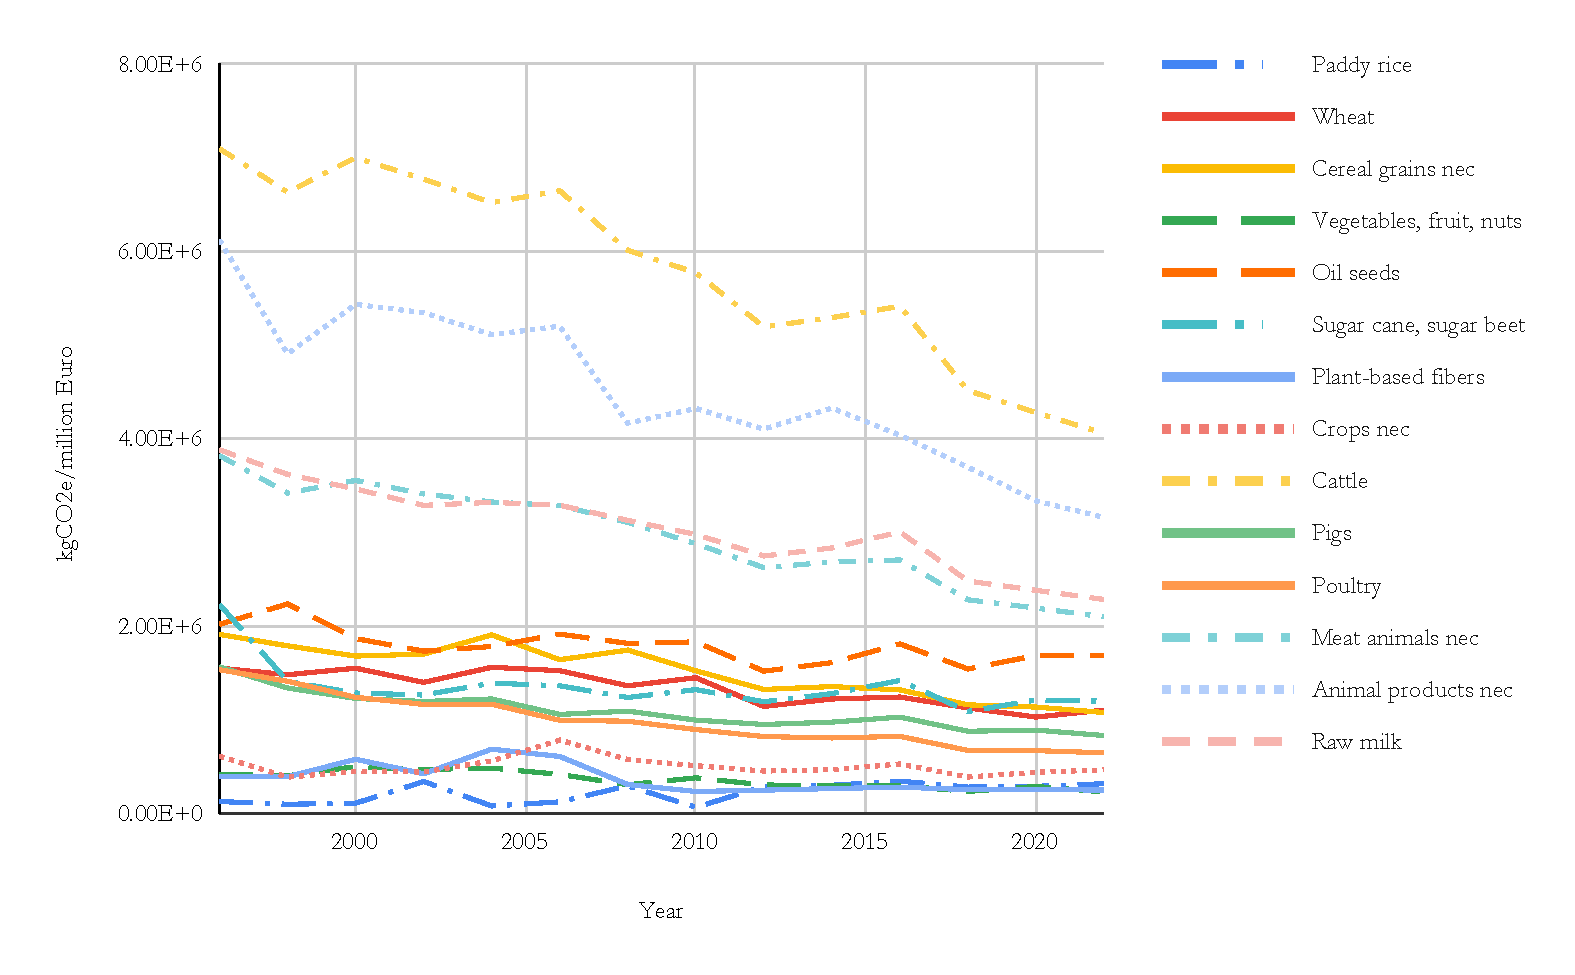
\includegraphics[width=0.7\textwidth]{raw_multipliers}
\caption{The multipliers per sector for French agriculture 1996 - 2022.}\label{fig:rawmultipliers} 
\end{figure}


\begin{figure}[H]
\centering
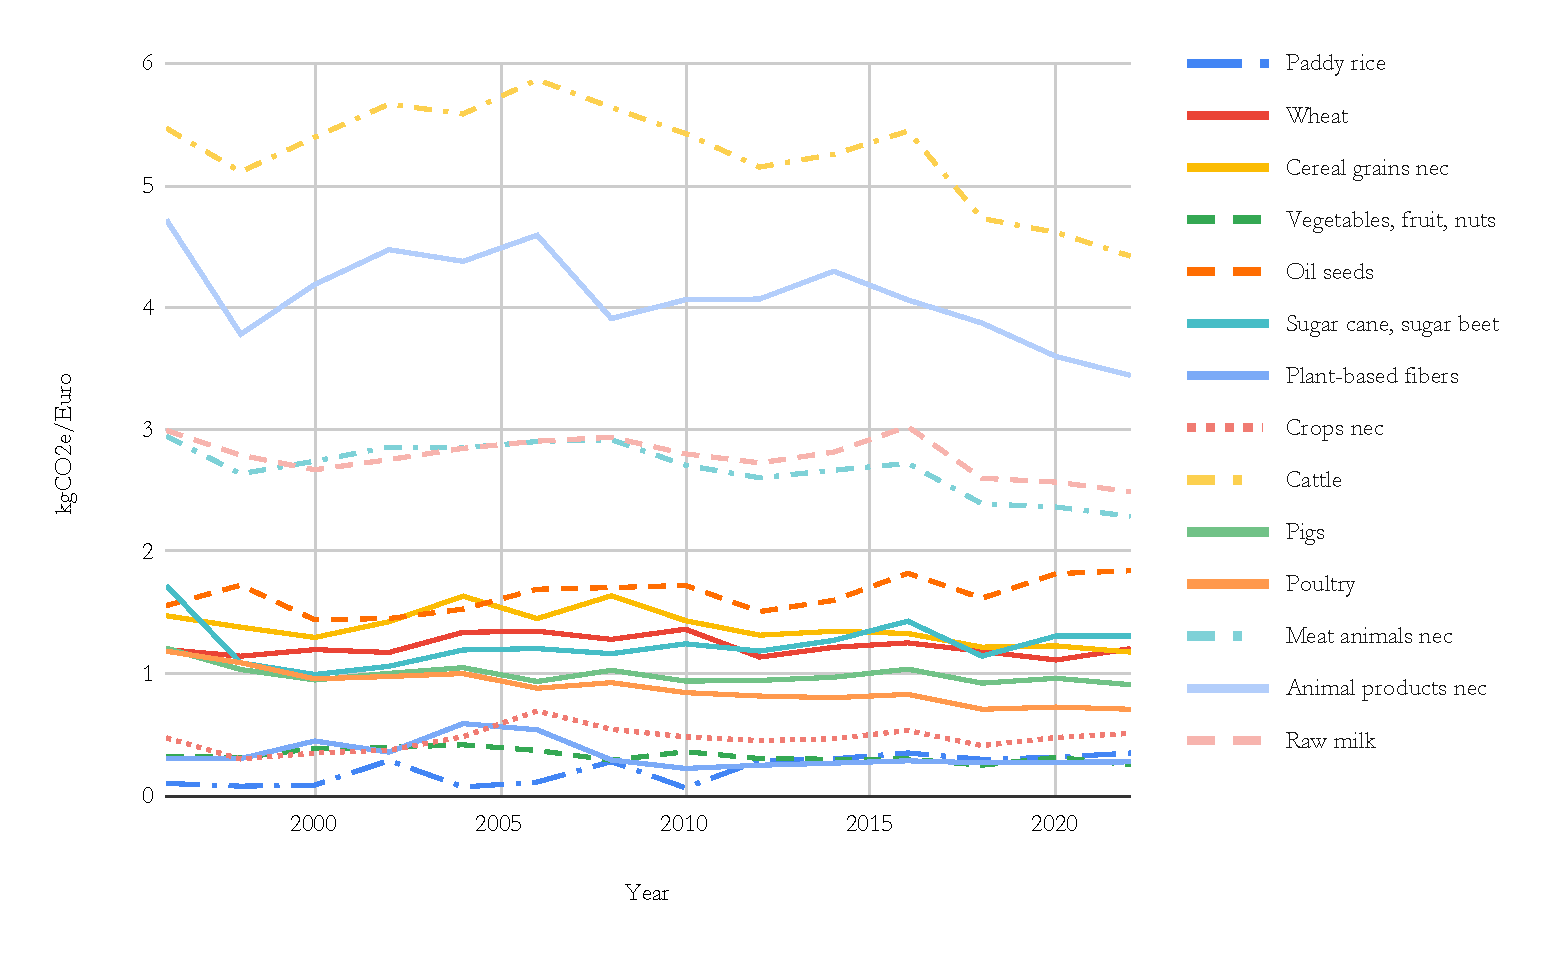
\includegraphics[width=0.7\textwidth]{inflated_adjusted}
\caption{The inflation-adjusted multipliers per sector for French agriculture 1996 - 2022}\label{fig:adjustedmultipliers} 
\end{figure}


\begin{figure}[H]
\centering
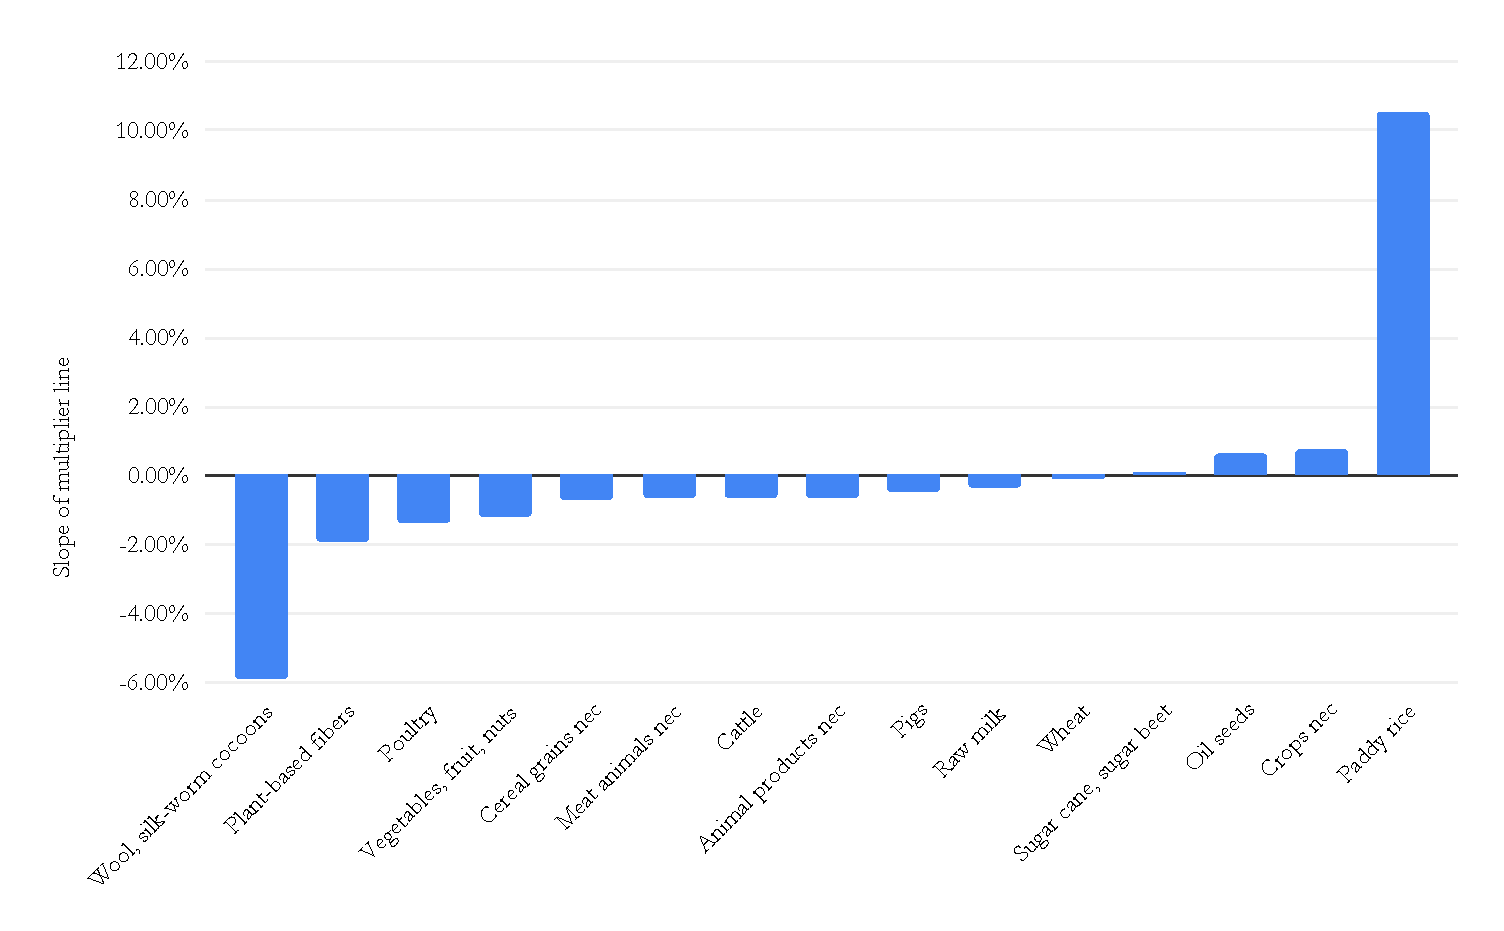
\includegraphics[width=0.9\textwidth]{slope}
\caption{The slope of the normalized multiplier line for each sector for the period 1996 - 2022}\label{fig:slope} 
\end{figure}


\section{Discussion}

\bibliography{IOreport}

\appendix

\section{Python code}

\begin{lstlisting}

# %%
# Load Libraries
import pymrio
import numpy as np
import pandas as pd

# Define Inputs
Country = 'FR'
charact_table = pd.read_csv('public_char_factors.csv',  sep='\t')
ghg = 'GHG emissions (GWP100) | Problem oriented approach: baseline (CML, 2001) | GWP100 (IPCC, 2007)'

years = [str(year) for year in [*range(1996, 2024, 2)]]

# %%
# Next we iterate over the year range
for year in years:
  currentpath = 'IOT_'+year+'_pxp.zip'
  # Load data
  print('Loading data for ', year)
  current_exio = pymrio.parse_exiobase3(path=currentpath)
  # Calculate system
  print('Calculating data for ', year)
  current_exio.calc_all()
  # Characterize system
  print('Characterizing data for ', year)
  current_multiplier = current_exio.impacts.M[Country].loc[[ghg]].iloc[:, 0:15]
  # Store relevant multipliers
  current_multiplier.to_excel('multipliers'+year+'.xlsx')
  print('Calculation for year ', year, ' complete')
  
\end{lstlisting}

\end{document}